\documentclass[aspectratio=169]{beamer}

%% Juego de caracteres usado en el archivo fuente: UTF-8
\usepackage{ucs}
\usepackage[utf8x]{inputenc}
\uselanguage{spanish}
%Para la identación del español
\usepackage[spanish]{babel}
\usepackage{animate}
\setbeamercovered{dynamic}
\useinnertheme{rectangles}

% There are many different themes available for Beamer. A comprehensive
% list with examples is given here:
% http://deic.uab.es/~iblanes/beamer_gallery/index_by_theme.html
% You can uncomment the themes below if you would like to use a different
% one:
%\usetheme{AnnArbor}
%\usetheme{Antibes}
%\usetheme{Bergen}
%\usetheme{Berkeley}
%\usetheme{Berlin}
%\usetheme{Boadilla}
%\usetheme{boxes}
%\usetheme{CambridgeUS}
%\usetheme{Copenhagen}
%\usetheme{Darmstadt}
%\usetheme{default}
%\usetheme{Frankfurt}
%\usetheme{Goettingen}
%\usetheme{Hannover}
%\usetheme{Ilmenau}
%\usetheme{JuanLesPins}
%\usetheme{Luebeck}
\usetheme{Madrid}
%\usetheme{Malmoe}
%\usetheme{Marburg}
%\usetheme{Montpellier}
%\usetheme{PaloAlto}
%\usetheme{Pittsburgh}
%\usetheme{Rochester}
%\usetheme{Singapore}
%\usetheme{Szeged}
%\usetheme{Warsaw}

%Para la identación del español
\usepackage[spanish]{babel}

\title{Infraestructura de red de nodos cifradores/descifradores AES basada en ApSoC}

% A subtitle is optional and this may be deleted
%\subtitle{Optional Subtitle}

\author{Jesús Rodríguez Heras}
% - Give the names in the same order as the appear in the paper.
% - Use the \inst{?} command only if the authors have different
%   affiliation.

%\institute[Escuela Superior de Ingeniería] % (optional, but mostly needed)
%{
%  \inst{1}%
%  Department of Computer Science\\
%  University of Somewhere
%  \and
%  \inst{2}%
%  Department of Theoretical Philosophy\\
%  University of Elsewhere}
% - Use the \inst command only if there are several affiliations.
% - Keep it simple, no one is interested in your street address.

\date{24 de septiembre de 2020}
% - Either use conference name or its abbreviation.
% - Not really informative to the audience, more for people (including
%   yourself) who are reading the slides online

%\subject{Theoretical Computer Science}
% This is only inserted into the PDF information catalog. Can be left
% out. 

% If you have a file called "university-logo-filename.xxx", where xxx
% is a graphic format that can be processed by latex or pdflatex,
% resp., then you can add a logo as follows:

% pgfdeclareimage[height=0.5cm]{university-logo}{university-logo-filename}
% \logo{\pgfuseimage{university-logo}}

% Delete this, if you do not want the table of contents to pop up at
% the beginning of each subsection:
\AtBeginSection[]
{
  \begin{frame}<beamer>{Índice}
    \tableofcontents[currentsection]
  \end{frame}
}
%\AtBeginSubsection[]
%{
%	\begin{frame}<beamer>{Índice}
%	\tableofcontents[currentsection,currentsubsection]
%\end{frame}
%}

% Let's get started
\begin{document}

\begin{frame}
  \titlepage
%  \begin{center}
%  Luis Gutiérrez Flores\\
%Nicolás Ruiz Requejo\\
%Jesús Rodríguez Heras\\
%Arantzazu Otal Alberro\\
%Alejandro Segovia Gallardo\\
%Alejandro José Caraballo García\\
%Gabriel Fernando Sánchez Reina	
%  \end{center}
  
\end{frame}

\begin{frame}{Índice}
%\small
\tableofcontents
\end{frame}
%\normalsize

\section{Introducción}
\subsection{Objetivos}
\begin{frame}{Objetivos}
%\textcolor{red}{Aquí hablaríamos de lo que son los objetivos al igual que en la memoria pero mucho más esquemático para que me permita hablar más que lo que es la lectura de la diapositiva por parte del tribunal}
Los objetivos generales de este proyecto son los siguientes:
\begin{itemize}
	\item Diseñar red de nodos basada en la tecnología ApSoC.
	\item Establecer comunicación entre nodos de la red.
	\item Cada nodo aportará información a un fichero común de forma secuencial.
\end{itemize}
\end{frame}

\subsection{Descripción}
\begin{frame}{Descripción}
%\textcolor{red}{ARM y FPGA en el mismo circuito integrado que permite programar cualquier periférico hardware y controlarlo a través del procesador ARM. Hablar más de lo que es la comunicación en red gracias al ARM y de la FPGA.}
\begin{block}{Nodos}
	Los nodos de la red serán tarjetas de desarrollo Zybo Zynq 7010.
\end{block}
\begin{figure}[h]
	\centering
	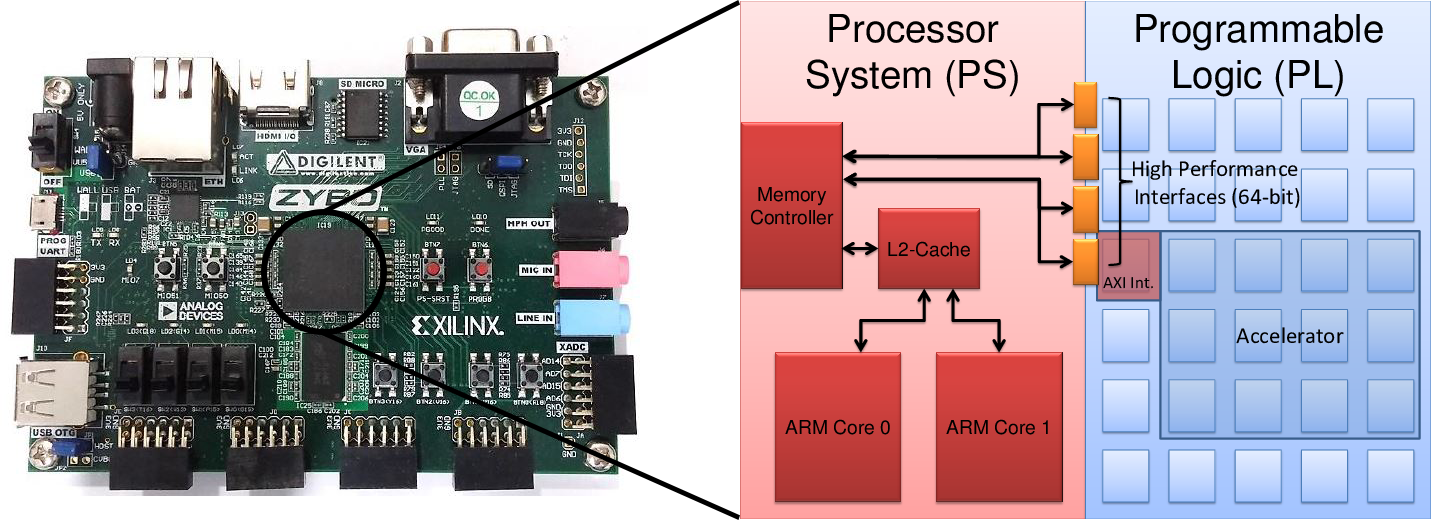
\includegraphics[scale=0.25]{Fotos/ZyboDescripcion.png}
\end{figure}
\begin{center}
	Fuente: Artículo ``Implementing high-performance, low-power FPGA-based optical flow accelerators in C.'', escrito por: Joshua Scott Monson.
\end{center}
\end{frame}



\subsection{Alcance}
\begin{frame}{Alcance}
\begin{block}{Infraestructura de red}
	\begin{itemize}
		\item Instalación de Linux sobre el núcleo ARM de las tarjetas.
		\item Interconexión física de los elementos de la red.
		\item Desarrollo de scripts para automatizar la comunicación y el agregado de información por parte de cada nodo.
		\item Creación y ejecición de pruebas.
	\end{itemize}
\end{block}
\end{frame}
%\begin{frame}{Alcance}
%\textcolor{red}{Hablamos de lo que consiste el alcance, como en la memoria.\\Realmente lo he estructurado todo como en la memoria con la idea de tener una guía que seguir y que todo vaya, más o menos, cogido de la mano.}
%El proyecto contará con los siguientes apartados:
%\begin{itemize}
%	\item 
%\end{itemize}
%\end{frame}

\section{Metodología}
%\subsection{Marco teórico}
%\begin{frame}{Marco teórico}
%\begin{itemize}
%	\item El punto de partida de este proyecto son las tarjetas de desarrollo Zybo Zynq 7010 que actuarán como nodos de la red.
%	\item Se establecerán comunicaciones entre ellas para enviar un fichero recolector de información.
%\end{itemize}
%\end{frame}

\subsection{Tecnologías a utilizar}
\begin{frame}{Tecnologías a utilizar}
\begin{block}{Componentes}
	\begin{itemize}
		\item Ordenador central (monitor).
		\item Tarjeta Zybo Zynq 7010.
		\item Switch.
	\end{itemize}
\end{block}
%\textcolor{red}{Poner un simbolito de debian al lado de cada elemento dentro de una tarjeta SD. Poner un simbolito de un fichero de texto numerado al lado de cada elemento.}
\begin{figure}[h]
\centering
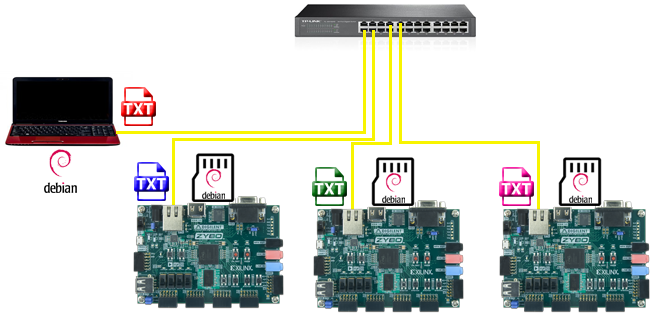
\includegraphics[scale=0.4]{Fotos/RedCompletaTecnologias.png}
\end{figure}
\end{frame}

\subsection{Análisis del sistema}
%\begin{frame}{Análisis del sistema}
%\begin{block}{Ordenador central}
%	Creará el fichero inicial y será el punto de partida y final de la cadena.
%\end{block}
%\begin{block}{Nodos}
%	Tendrán instalado un sistema operativo Linux para la gestión de ficheros y las funcionalidades de red.
%\end{block}
%\begin{block}{Switch}
%	No tendrá ninguna configuración adicional.
%\end{block}
%\end{frame}

\begin{frame}{Análisis del sistema}
%	\textcolor{red}{Comentar que el sistema operativo del portátil es debian (x86). Y, el de las tarjetas puede ser Xilliunx o debian compilado para ARM, pero que hay que incluir el devicetree (fichero de linux que recopila los dispositivos). De momento, no incluye ningún driver. Como ya tenemos un sistema operativo Linux, nos permitirá la creación de scripts en bash y la comunicación mediante SSH. SSH porque permite comunicación serie mediante consola a través de la red y de forma cifrada. De tal forma que la información que añade cada nodo al fichero, queda cifrada durante el proceso de comunicación. Gracias a SCP (utilidad de SSH) podemos enviar ficheros entre dispositivos que estarán cifrados durante el proceso de comunicación. Contar también que usamos el comando stat. Añadir una foto con los directorios de los nodos para que se vea la secuencia.}
	\begin{itemize}
		\item Sistema operativo del ordenador central: Debian 9 Stretch.
		\item Sistema operativo de las tarjetas de desarrollo: Debian 8 Jessie (compilado para ARM en tarjeta micro SD).
		\item Uso de SSH en las comunicaciones.
		\item Uso de SCP para el envío de ficheros.
		\item Comprobación de directorios con el comando \texttt{stat}.
	\end{itemize}
\end{frame}

\begin{frame}{Análisis del sistema}
%Ahora vamos a ver las tareas que realiza cada nodo de forma individual. Se centra en tres tareas.
	Las tareas a realizar por cada nodo se realizan en los siguientes scripts:
	

\begin{columns}
	\column{0.45\textwidth}
		\begin{block}{\texttt{Recibiendo.sh} (Nodo)}
			Comprobar (stat) recepción del fichero de texto.
		\end{block}
		\begin{block}{\texttt{Cristian.sh} (Nodo)}
			Comprobar (stat) el directorio de trabajo.
			Añade la información local.
		\end{block}
		\begin{block}{\texttt{Enviando.sh} (Nodo)}
			Comprobar (stat) el directorio de envío.
			Comprobar la conexión del siguiente nodo (ping).
			Envía el fichero mediante SCP.
		\end{block}
	\column{0.55\textwidth}
		\begin{figure}[h]
			\centering
			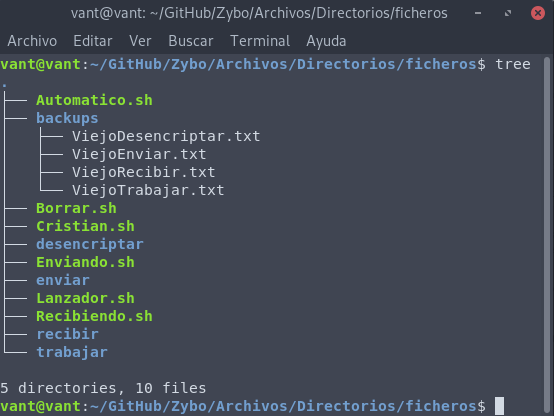
\includegraphics[scale=0.56]{Fotos/Tree.png}
		\end{figure}
\end{columns}
\end{frame}

\begin{frame}{Análisis del sistema}
%	\textcolor{red}{Para que el sistema trabaje de forma autonoma se necesita que la red funcione de forma desatendida, para ello se han programado una serie de scripts que serán lanzados mediante la herramienta cron. Esta herramienta permite programar mediante eventos o temporalmente la ejecución de scripts.}
	\begin{block}{¿Cómo conseguir la automatización?}
		\begin{itemize}
			\item Lanzamiento de scripts al inicio del Sistema Operativo con la herramienta \texttt{cron}.
			\item Evitar la saturación del arranque del Sistema Operativo.
			\item Periodicidad de las comprobaciones de los directorios de trabajo y lanzamiento de scripts.
		\end{itemize}
	\end{block}
\end{frame}

\begin{frame}{Análisis del sistema}

\begin{columns}
	\column{0.45\textwidth}
	Para evitar saturar el arranque del sistema, hacemos una planificación del arranque de cada tarjeta con los siguientes scripts:
	\begin{block}{\texttt{Lanzador.sh} (Nodo)}
		Es ejecutado por la herramienta cron del sistema operativo.
		Ejecuta el script \texttt{Automatico.sh}.
	\end{block}
	\begin{block}{\texttt{Automatico.sh} (Nodo)}
		Periódicamente, ejecuta los scripts \texttt{Recibiendo.sh}, \texttt{Cristian.sh} y \texttt{Enviando.sh}.
		El parámetro de tiempo seleccionado es de un segundo. %Se considera tiempo suficiente para que el resto de acciones hayan tenido lugar. Hay que justificar este segundo.
	\end{block}
	\column{0.55\textwidth}
	\begin{figure}[h]
		\centering
		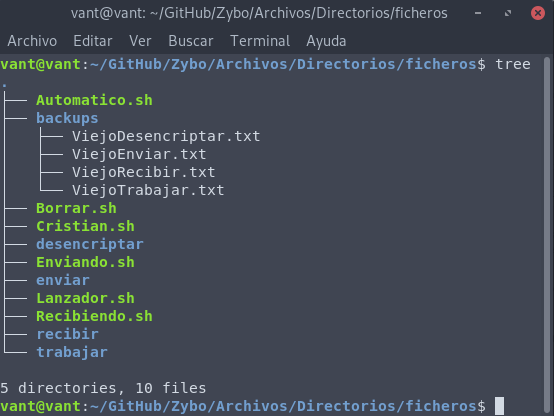
\includegraphics[scale=0.56]{Fotos/Tree.png}
	\end{figure}
\end{columns}
\end{frame}

\begin{frame}{Análisis del sistema}
	La secuencia de trabajo de estos scripts será la siguiente:
	\begin{figure}[h]
		\centering
		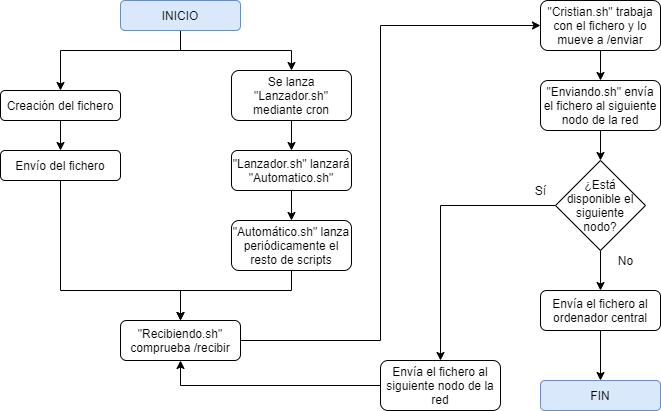
\includegraphics[scale=0.45]{Fotos/CadenaScriptsAncho.png}
	\end{figure}
\end{frame}

\subsection{Diseño y desarrollo}
\begin{frame}{Diseño y desarrollo}
\begin{itemize}
	\item Todos los dispositivos de la red han de estar conectados al switch y tener una IP fija.
	\item El proceso de comunicación se inicia en el ordenador central (monitor).
	\item Los nodos reciben el fichero, añaden información y lo envían al siguiente nodo de la red.
	\item El proceso de comunicación finaliza cuando el fichero es recibido por el monitor.
\end{itemize}
\end{frame}

\subsection{Pruebas del sistema}
\begin{frame}{Pruebas del sistema}
%	\textcolor{red}{Enumerar las dos pruebas, la de conexión de red y la de comunicación completa. Como usuario del sistema lanzo Inicio.sh y se ejecuta la de red. Y la otra se verá en directo.}
	Tendremos dos pruebas principales:
	\begin{itemize}
		\item Prueba de conexión de red con el lanzamiento de \texttt{Inicio.sh} por parte del monitor.
		\item Prueba de comunicación del sistema completamente automatizado.
	\end{itemize}
\end{frame}
%\begin{frame}{Pruebas del sistema}
%\begin{block}{Prueba de conexión}
%	Lanzamos el script \texttt{Inicio.sh} en el ordenador central.
%	\begin{figure}[h]
%		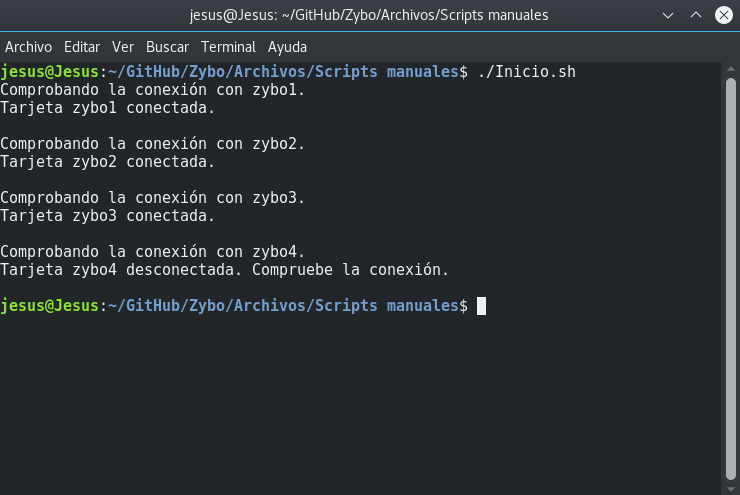
\includegraphics[scale=0.3]{Fotos/Prueba_Inicio_sh.png}
%	\end{figure}
%\end{block}
%\end{frame}
%
%\begin{frame}{Pruebas del sistema}
%\begin{block}{Prueba de funcionamiento (I)}
%	Creamos el fichero de pruebas y lo enviamos al primer nodo de la red.
%	\begin{figure}[h]
%		\centering
%		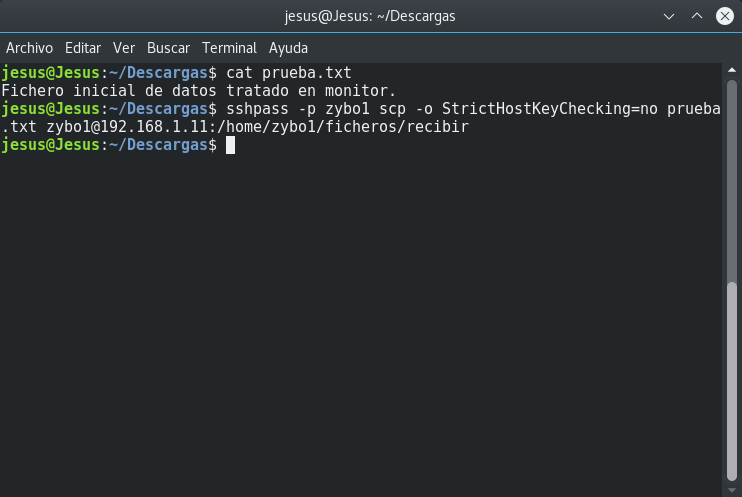
\includegraphics[scale=0.3]{Fotos/Fichero_inicial_en_PC.png}
%	\end{figure}
%\end{block}
%\end{frame}
%
%\begin{frame}{Pruebas del sistema}
%\begin{block}{Prueba de funcionamiento (II)}
%	Comprobamos el paso del fichero por la tarjeta Zybo.
%	\begin{figure}[h]
%		\centering
%		\includegraphics[scale=0.3]{Fotos/Fichero_en_zybo1.png}
%	\end{figure}
%\end{block}
%\end{frame}
%
%\begin{frame}{Pruebas del sistema}
%\begin{block}{Prueba de funcionamiento (III)}
%	Una vez completada la cadena de nodos, comprobamos el fichero en el monitor.
%	\begin{figure}[h]
%		\centering
%		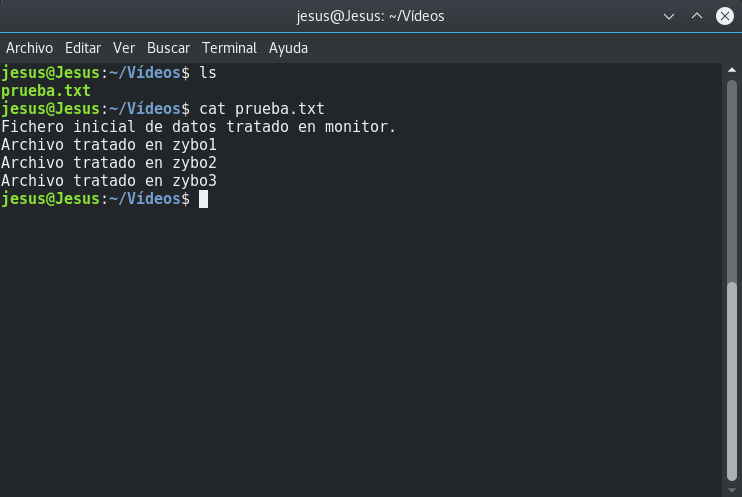
\includegraphics[scale=0.3]{Fotos/Fichero_final_en_PC.png}
%	\end{figure}
%\end{block}
%\end{frame}

\section{Conclusiones y trabajo futuro}
\subsection{Conclusiones}
\begin{frame}{Conclusiones}
\begin{itemize}
	\item Aunque la red se pensó inicialmente para un cifrado/descifrado AES, realmente, puede usarse para cualquier tipo de módulo hardware implementado en la FPGA de la tarjeta de desarrollo Zybo Zynq 7010, como por ejemplo, el tratamiento de imágenes.
	\item El sistema está preparado para soportar tantos nodos de red como capacidad física tenga la red usada.
\end{itemize}
\end{frame}

\begin{frame}{Conclusiones}
\begin{block}{Escenario de trabajo 1}
	Todos los nodos están conectados correctamente a la red.
	\begin{figure}[h]
		\centering
		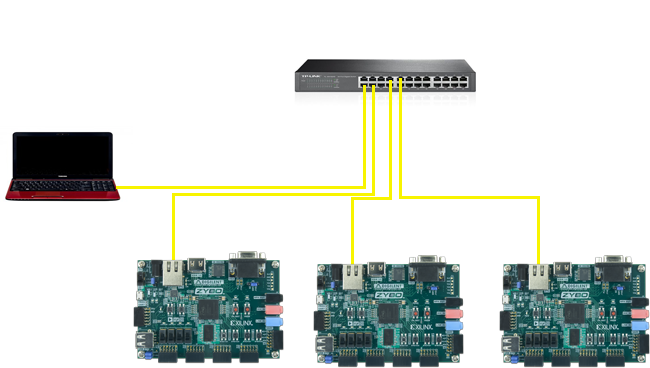
\includegraphics[scale=0.4]{Fotos/RedCompleta.png}
	\end{figure}
\end{block}
\end{frame}

\begin{frame}{Conclusiones}
\begin{block}{Escenario de trabajo 2}
	Un nodo intermedio se encuentra desconectado.
	\begin{figure}[h]
		\centering
		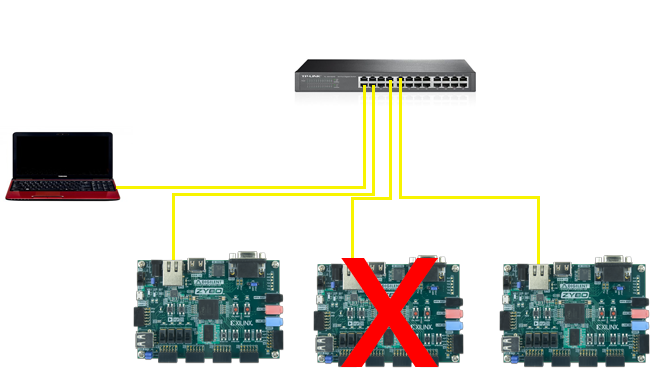
\includegraphics[scale=0.4]{Fotos/RedSinNodo2.png}
	\end{figure}
\end{block}
\end{frame}

\begin{frame}{Conclusiones}
\begin{block}{Escenario de trabajo 3}
	El primer nodo está desconectado.
	\begin{figure}[h]
		\centering
		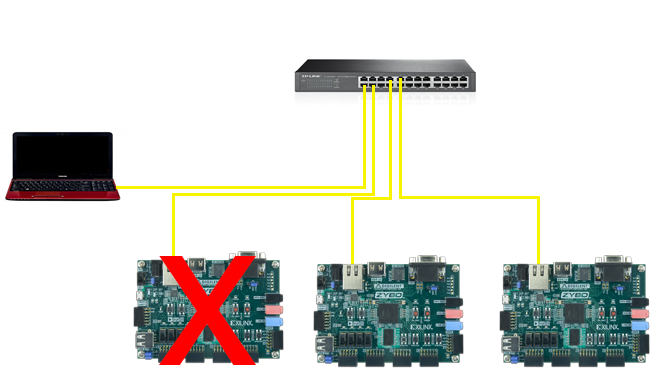
\includegraphics[scale=0.4]{Fotos/RedSinNodo1.png}
	\end{figure}
\end{block}
\end{frame}

\subsection{Aclaraciones}
\begin{frame}{Aclaraciones}
	\begin{itemize}
		\item Hay un cifrado en la comunicación ya que se usa el protocolo SSH y SCP para las comunicaciones y envío de ficheros.
		\item No hay cifrado local de la información del nodo aportado por el Trabajo de Fin de Grado de Cristian Ambrosio Costoya por incompatibilidad con el Trabajo de Fin de Grado de Gabriel Fernando Sánchez Reina el cual debía proporcionar el driver Linux para comunicarse con este módulo cifrador.
	\end{itemize}
\end{frame}

\subsection{Trabajo futuro}
\begin{frame}{Trabajo futuro}
\begin{itemize}
	\item Cambiar cadena de conexiones a aleatorio.
	\item Completar el trabajo de cifrado/descifrado incluyendo el IP cifrador/descifrador AES de Cristian Ambrosio Costoya y el driver de Gabriel Fernando Sánchez Reina.
	\item Implementación de un módulo IEEE 802.11 para conexiones inalámbricas de todos los nodos de la red.
\end{itemize}
\end{frame}

\end{document}


